\section{Introduction}

The rapid development of text-to-video models has been phenomenal, driven by both the Transformer architecture~\citep{vaswani2017attention} and diffusion model~\citep{ho2020denoising}. 
Early attempts to pretrain and scale Transformers to generate videos from text have shown great promise, such as CogVideo~\citep{hong2022cogvideo} and Phenaki~\citep{villegas2022phenaki}. 
Meanwhile, diffusion models have recently made exciting advancements in multimodal generation, including video generation~\citep{singer2022make, ho2022imagen}. 
By using Transformers as the backbone of diffusion models, i.e., Diffusion Transformers (DiT) \citep{peebles2023scalable}, text-to-video generation has reached groundbreaking levels, as evidenced by the impressive Sora showcases~\citep{sora}.  


Despite these rapid advancements in DiTs, it remains technically unclear how to achieve long-term consistent video generation. 
Challenges such as efficiently modeling video data, effectively aligning videos with text semantics, as well as constructing the high-quality text-video pairs for model training have thus far been largely unaddressed. 


In this work, we train and introduce \model, a set of large-scale diffusion transformer models designed for generating long-term, temporally consistent videos. 
We address the challenges mentioned above by developing a 3D variational Autoencoder (VAE), an expert Transformer, and a video data filtering and captioning pipeline, respectively. 
First, to efficiently consume video data, we design and train a 3D causal VAE that compresses the video along both spatial and temporal dimensions. 
Compared to unfolding a video into a one-dimensional sequence in the pixel space, this strategy helps significantly reduce the sequence length and associated training compute. 
Unlike previous video models~\citep{blattmann2023stable} that often use a 2D VAE to encode each frame separately, the 3D VAE helps prevent flicker in the generated videos, that is, ensuring continuity among frames. 

%\begin{wrapfigure}{r}{0.5\textwidth}
% \begin{figure}
% \centering
% 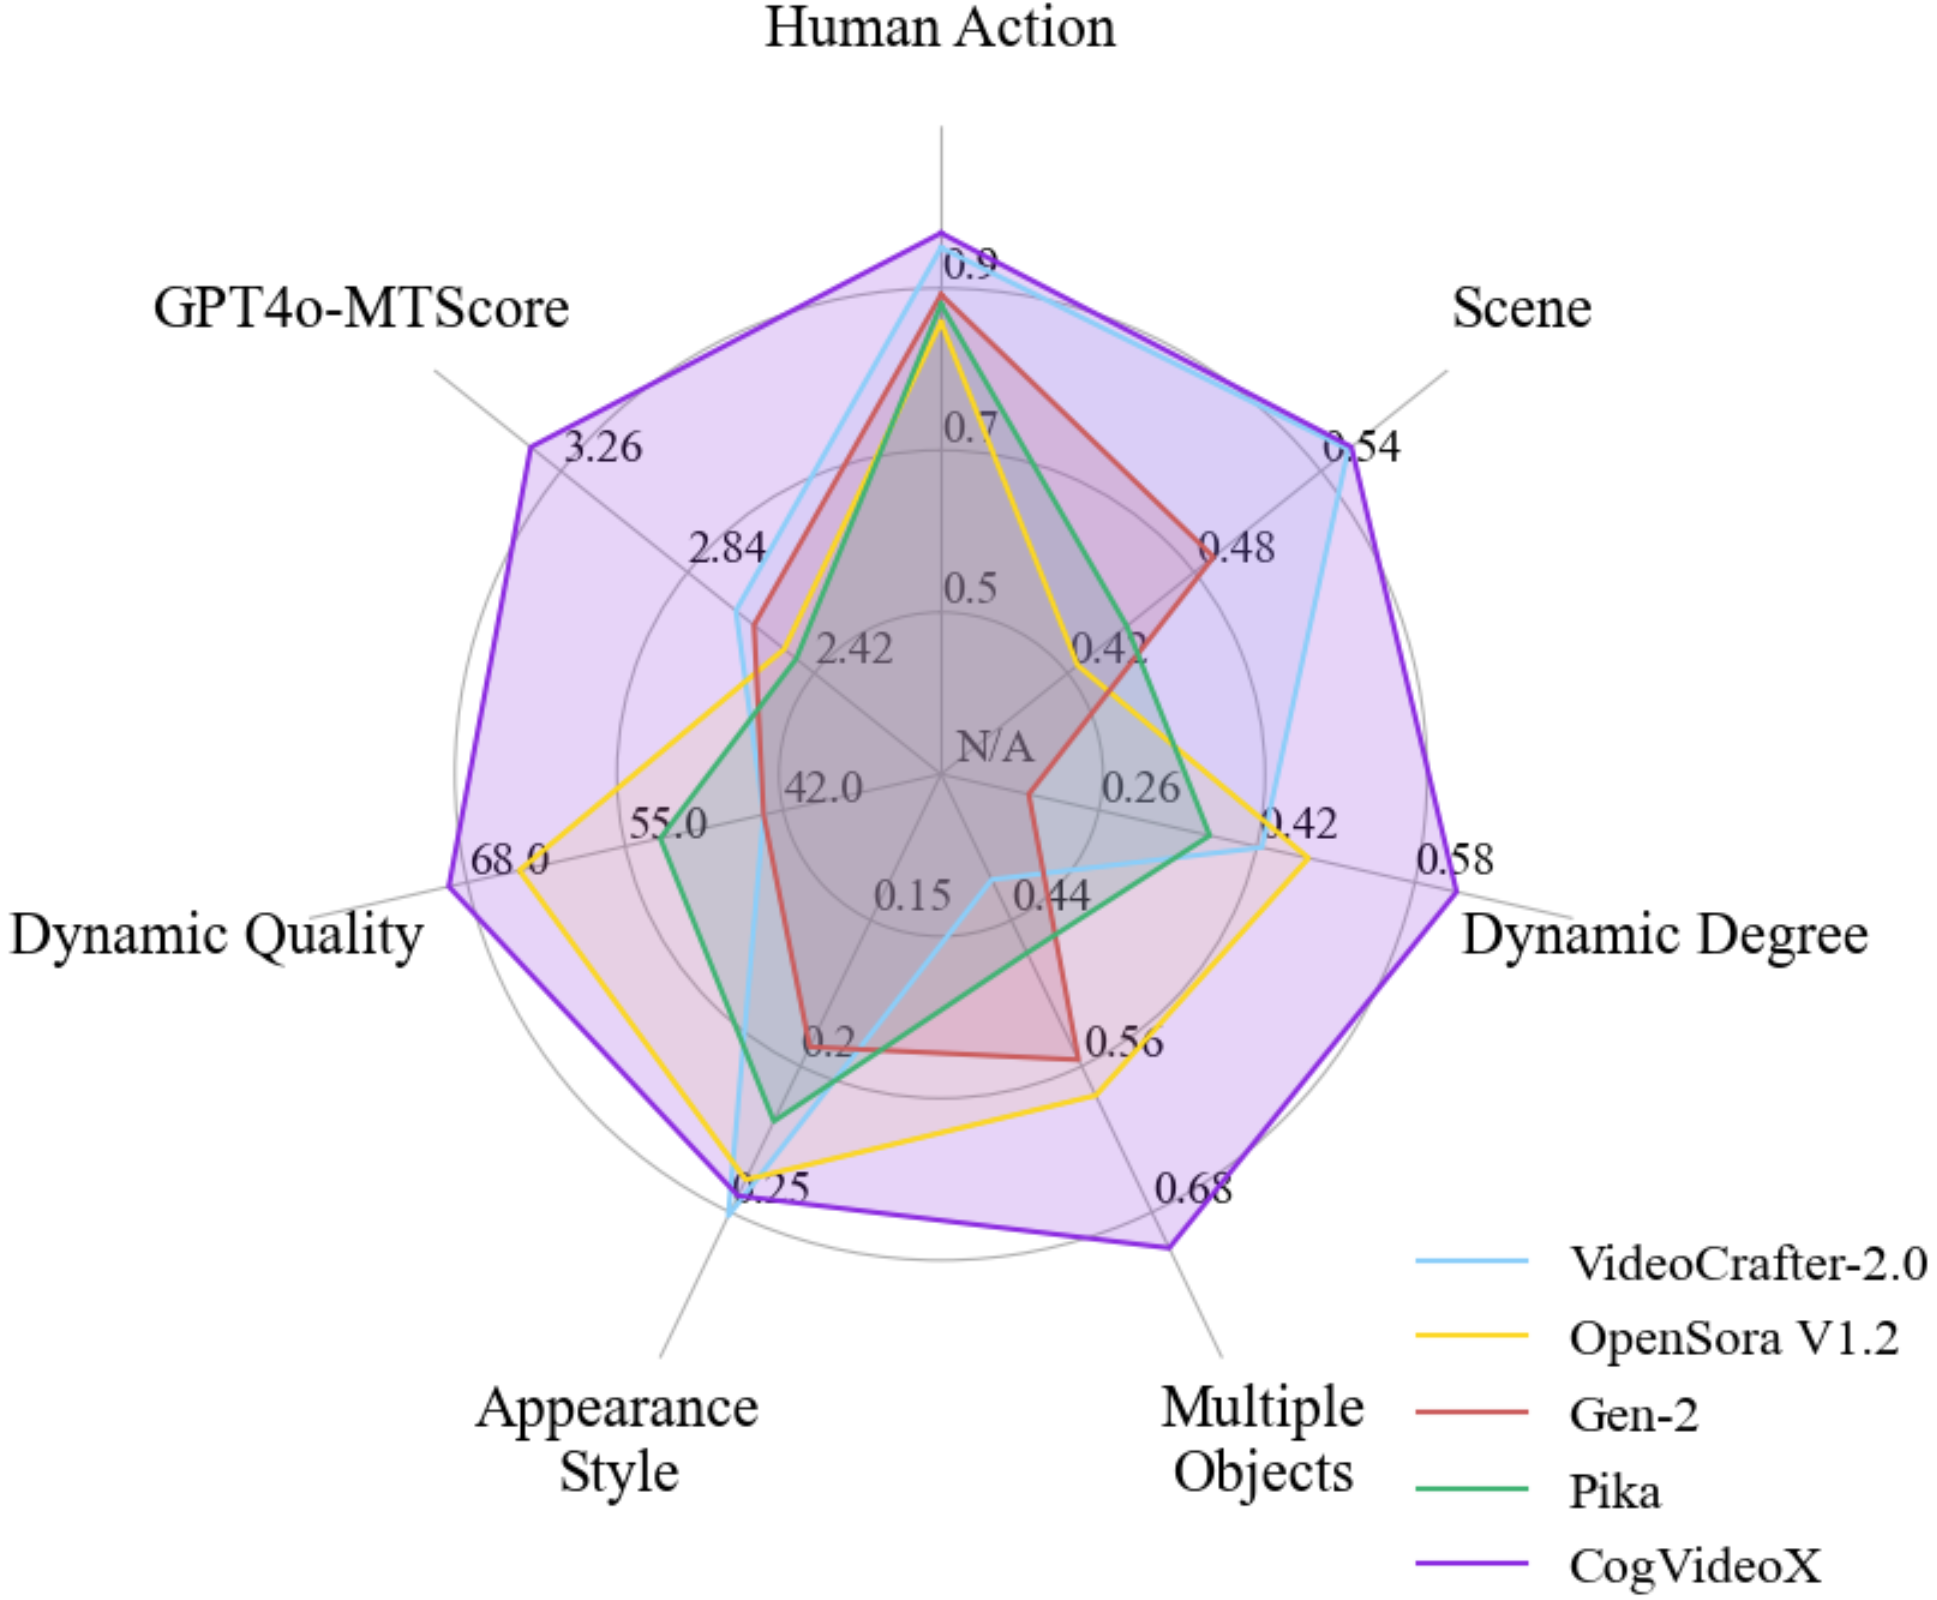
\includegraphics[width=0.7\linewidth]{images/bench_eval8.png}
% \caption{The performance of openly-accessible text-to-video models in different aspects.}
% \label{fig:radar}
% % \vspace{-10mm}
% %\end{wrapfigure}

% \end{figure}

%  With 2B
\begin{figure}
\centering
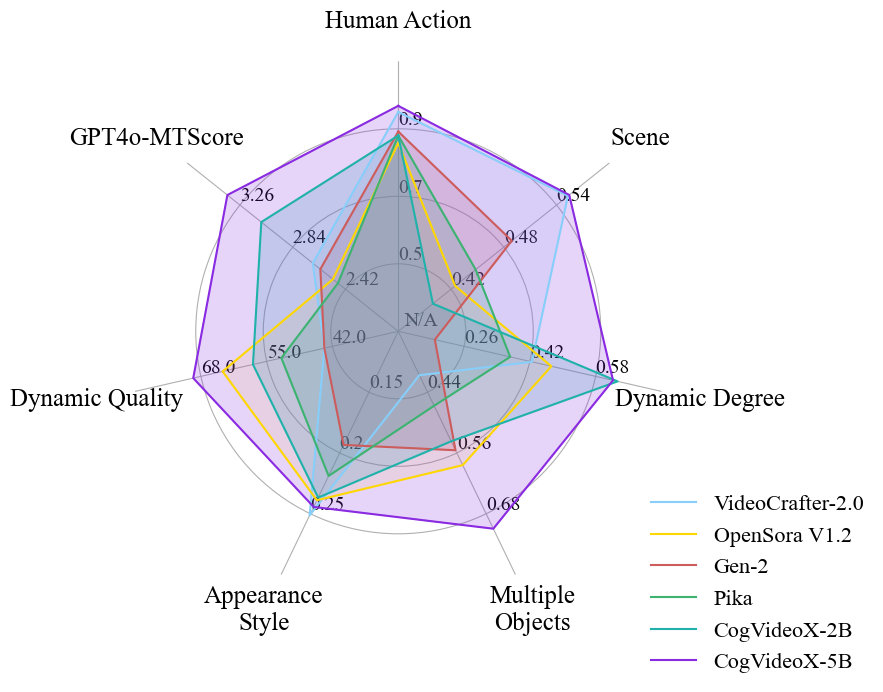
\includegraphics[width=0.7\linewidth]{images/bench_eval9.png}
\caption{The performance of openly-accessible text-to-video models in different aspects.}
\label{fig:radar}
% \vspace{-10mm}
%\end{wrapfigure}

\end{figure}



Second, to improve the alignment between videos and texts, we propose an expert Transformer with  expert adaptive LayerNorm to facilitate the fusion between the two modalities. 
To ensure the temporal consistency in video generation and  capture large-scale motions, we propose to use 3D full attention to comprehensively model the video along both temporal and spatial dimensions. 

Third, as most video data available online lacks accurate textual descriptions, we develop a video captioning pipeline capable of accurately describing video content. 
This pipeline is used to generate new textual descriptions for all video data, which significantly enhances \model's ability to grasp precise semantic understanding. 
%In addition, we also train an end-to-end video understanding model for 

In addition, we adopt and design progressive training techniques, including mixed-duration training and resolution progressive training, to further enhance the generation performance and stability of \model. Furthermore, we propose Explicit Uniform Sampling, which stablizes the training loss curve and accelerates convergence by setting different timestep sampling intervals on each data parallel rank.

Both machine and human evaluations suggest that \model outperforms well-known public models. 
Figure \ref{fig:radar} shows the performance of \model in different aspects. 

\model is an ongoing attempt to advance text-to-video generation. 
To facilitate further developments, we open-source the model weight of part of \model and the 3D VAE, and we plan to release future and larger models as well. 
Now open-sourced \model is capable of generating 720$\times$480 videos of six seconds with eight frames per second. 
It can be publicly accessed from \url{https://github.com/THUDM/CogVideo}. 


 







\hide{%%%%%%% 

\section{Introduction}

In recent years, diffusion models have made groundbreaking advancements in multimodal generation, such as image, video, speech and 3D generation. Among these, video generation is a rapidly evolving field and being extensively explored. Given the successful experiences with Large Language Models (LLMs), comprehensive scaling up of data volume, training iterations, and model size consistently enhances model performance. Additionally, there is more mature scaling experience with transformers compared to UNet. And DiT \citep{peebles2023scalable} has shown that transformers can effectively replace UNet as the backbone of diffusion models. Thus, transformer is a better choice for video generation.
However, long-term consistent video generation remains a significant challenge.  % 第一段介绍任务重要性和我们工作的亮点,例如开源。DiT的讨论不应该在这里

The first challenge is that constructing a web-scale video data pipeline is considerably more difficult than for textual data. Video data is extremely diverse in distribution, quality varies greatly, and simple rule-based filtering is often insufficient for effective data selection. Consequently, processing video data is both time-consuming and highly complex.
There are numerous meaningless unrealistic videos, such as poor-quality edits and computer screen recordings. And many videos are difficult to watch normally, such as those with excessively shaky cameras. These types of data are harmful to the generative model's ability to learn genuine dynamic information. They need to be meticulously processed and filtered out to ensure the quality of the training dataset.

Additionally, most video data available online lacks accurate textual descriptions, significantly limiting the model's ability to grasp precise semantic understanding. To address this issue, we trained a video understanding model capable of accurately describing video content. We use it to generate new textual descriptions for all video data. 
To advance the field of video generation, we have decided to open-source this description model.

The high training cost is another significant challenge. If the video is unfolded into a one-dimensional sequence in the pixel space, the length would be extraordinarily long. To keep the computational cost within a feasible range, we trained a 3D VAE that compresses the video along both spatial and temporal dimensions. Additionally,  unlike previous video models that use a 2D VAE to encode each frame separately, 3D VAE ensures continuity among frames so that the generated videos do not flicker. 

Moreover, to improve the alignment between videos and texts, we propose an expert transformer to facilitate the interaction between the two modalities. Then, to ensure the consistency of video generation and to capture large-scale motions, it is necessary to comprehensively model the video along both temporal and spatial dimensions. Therefore, we opt for 3D full attention, as detailed in Section~\ref{sec:expert-transformer}.



}